\documentclass[a4paper, 12pt]{article}
\usepackage[utf8]{inputenc}
\usepackage[english,russian]{babel}
\usepackage[warn]{mathtext}
\usepackage{graphicx}
\usepackage{float}
\usepackage{multirow}
\restylefloat{table}
\usepackage{amsmath}
\usepackage{floatflt}
\usepackage[T2A]{fontenc}
\usepackage[left=20mm, top=20mm, right=20mm, bottom=20mm, footskip=10mm]{geometry}

\tolerance 1414
\hbadness 1414
\emergencystretch 1.5em
\hfuzz 0.3pt        % размер максимального переполнения без warning'a
\widowpenalty=10000 % запрещает одиночную строку абзаца в начале страницы
\vfuzz \hfuzz
\raggedbottom       % если на странице мало содержимого, добавить пустое место в конце, а не в середине страницы



\begin{document}

\begin{titlepage}
	\centering
	\vspace{5cm}
	{\scshape\LARGE московский физико-технический институт (национальный исследовательский университет) \par}
	\vspace{6cm}
	{\scshape\Large Лабораторная работа 5.2 \par}
	{\huge\bfseries Спектрометрия $\alpha$-излучения с помощью полупроводникового детектора\par}
	\vspace{1cm}
	\vfill
\begin{flushright}
	{\large Б03-104}\par
	\vspace{0.3cm}
	{\LARGE Куланов Александр}
\end{flushright}
	

	\vfill


	Долгопрудный, 2023 г.
\end{titlepage}

\begin{itemize}
	\item \textbf{Цель работы:} C помощью кремниевого поверхностно-барьерного детектора измеряются спектры $\alpha$-частиц, испускаемых различными радиоактивными ядрами - ${ }^{226} \mathrm{Ra},{ }^{238} \mathrm{U},{ }^{241} \mathrm{Am} + ^{230} \mathrm{Th}$ и ${ }^{239} \mathrm{Pu}$. Исследуется тонкая структура $\alpha-$ излучения и последовательность радиоактивных распадов в семействе урана.
\end{itemize}

\section{Теоретические сведения}
К числу радиоактивных процессов относятся $\alpha$- и $\beta$-распады (в том числе и $K$-захват), $\gamma$-излучение, деление ядер, а также испускание запаздывающих нейтронов и протонов. В этой работе изучается $\alpha$-распад.\\
Энергию вылетающих из ядра $\alpha$-частиц легко подсчитать на основе законов сохранения. Если родительское (исходное) ядро имеет массу $M_1$, а дочернее (конечное) - $M_2$, то законы сохранения энергии и импульса записываются в форме

$$
\begin{gathered}
M_2 c^2=M_1 c^2+m_\alpha c^2+T_1+T_\alpha, \\
\mathrm{p}_1+\mathrm{p}_\alpha=0
\end{gathered}
$$

где $T_1$ и $\mathrm{p}_1$ - кинетическая энергия и импульс отдачи дочернего ядра, a $T_\alpha$ и $\mathrm{p}_\alpha$ - кинетическая энергия и импульс $\alpha$-частицы.

Ясно, что вылет $\alpha$-частицы из ядра возможен лишь в том случае, если разность энергий покоя родительского и дочернего ядра будет больше энергии покоя $\alpha$-частицы. В силу того, что реально $\alpha$-распад испытывают лишь тяжелые ядра с $A>200$, энергия отдачи ядра очень мала и фактически кинетическая энергия $\alpha$-частицы равна разности энергий покоя исходного и конечного ядер. Именно поэтому вылетающие $\alpha$-частицы имеют строго определенную энергию.

Однако экспериментально обнаружено, что энергетический спектр $\alpha$-частиц многих $\alpha$-активных ядер состоит из нескольких линий, одна из которых преобладающее. Дискретность линий и их относительная интенсивность объяснимы, поскольку, во-первых, $\alpha$-частицы могут испускаться ядром, находящимися в возбужденном состоянии (длиннопробежные $\alpha$-частицы), а во-вторых может происходить $\alpha$-распад из основного состояния родительского ядра на возбужденные состояния дочернего ядра (короткопробежные $\alpha$-частицы). Так как период полураспада для $\alpha$-частиц примерно в $10^5$ раз больше периода $\alpha$-распада, то интенсивность длиннопробежных $\alpha$-частиц очень мала.

Тяжелые ядра, как правило, в основном состоянии деформированы (исключением являются магические ядра). Это означает, что низколежащими состояниями являются вращательные полосы, и именно на эти состояния обычно и происходит распад родительского ядра, приводящий к появлению группы короткопробежных $\alpha$-частиц. Как известно, энергия вращательных уровней определяется выражением

$$
E_\text{вp}=\frac{\hbar^2}{2 \mathcal{I}} l(l+1).
$$

Тем самым измерение тонкой структуры энергетического спектра $\alpha$ частиц дает возможность определить момент инерции ядра $\mathcal{I}$.

Периоды полураспада $\alpha$-активных ядер очень сильно зависят от энергии вылетающих частиц. Экспериментально установленная зависимость (закон Гейгера-Нэттола) имеет вид:

\begin{equation}\label{eq:gey_net}
\lg T_{1 / 2}=\frac{a}{\sqrt{E_\alpha}}+b .
\end{equation}

Коэффициенты $a$ и $b$ очень слабо зависят от заряда ядра $Z$.
\section{Экспериментальная установка}
В состав экспериментальной установки входит альфа-спектрометр, форвакуумный насос и персональный компьютер. (Рис. \ref{fig:scheme})

\begin{figure}[h]
  \centering
  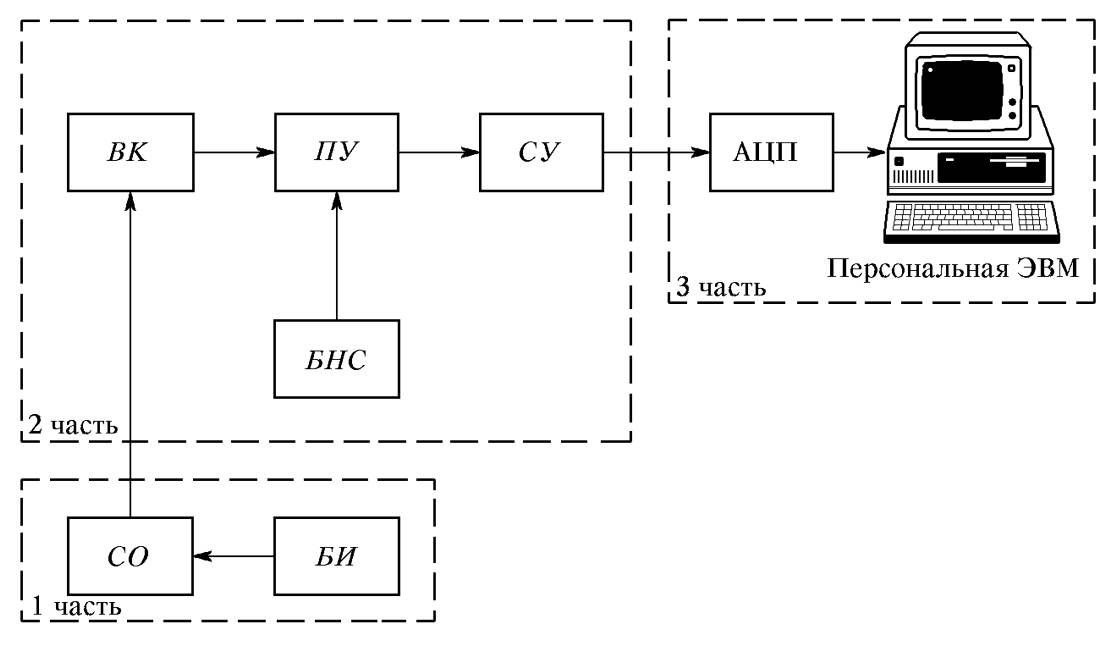
\includegraphics[width=0.8\textwidth]{ust.png}  \caption{Блок-схема спектрометра $\alpha$-излучения}
  \label{fig:scheme}
\end{figure}

Форвакуумный насос, соединенный с корпусом альфа-спектрометра вакуум-ным шлангом, откачивает измерительную камеру до давления 0,2 мм рт. ст.\\
Установка автоматически поддерживает давление в измерительной камере в рабочем диапазоне от 0,2 до 2,0 мм рт. ст. Откачка блокируется при разгер-метизации камеры. Соединение и отсоединение измерительной камеры с атмосферой осуществляется с помощью двух электромагнитных клапанов.\\

При использовании детектора в спектрометрических целях особое значение приобретает его разрешающая способность, т. е. ширина кривой распределения импульсов по амплитудам при строго постоянной энергии регистрируемых частиц. Форма такой кривой распределения обычно бывает близка к кривой ошибок (гауссовой кривой)

$$
W(U) d U=\frac{1}{\sqrt{2 \pi} \sigma} e^{-\left(U-U_0\right)^2 /\left(2 \sigma^2\right)} d U
$$

Распределение (5) имеет вид колокола с максимумом при $U=U_0$. Разрешающую способность спектрометра определяют по величине $\delta$ ширине кривой $W(U)$, измеренной на половине высоты. Энергетическим разрешением спектрометра обычно называют величину

$$
R=\frac{\delta}{U_0} \cdot 100 \% .
$$

Нетрудно найти связь между $\delta$ и $\sigma$:

$$
\delta=2 \sqrt{2 \ln 2} \sigma .
$$

Одной из основных причин, вызывающих разброс импульсов по амплитуде, является статистическая флуктуация числа электрондырочных пар, создаваемых падающей частицей. Среднее число пар $N$ равно

$$
N=E / E_{\mathrm{cp}},
$$

где $E$ - энергия, теряемая частицей в детекторе, а $E_{\mathrm{cp}}=3.6$ эВ - энергия, необходимая для создания пары электрон-дырка. Среднеквадратичное отклонение $\sigma$ равно

$$
\sigma=\sqrt{N}=\sqrt{E / E_{\mathrm{cp}}}
$$

Вклад флуктуаций числа пар в энергетическое разрешение

$$
R_{\text {флук }}=\frac{\sigma}{N} \cdot 100 \%=\sqrt{\frac{E_{\mathrm{cp}}}{E}} \cdot 100 \% .
$$

\section{Обработка результатов}
Сначала получим спектр $Ra$ и будем использовать его для калибровки. Номера каналов, соответствующих пикам: 1938, 2221, 2417, 3092. Этим пикам соответствуют энергии 4.784, 5.490, 6.002, 7.687 Мэв.
\begin{figure}[H]
	\centering
	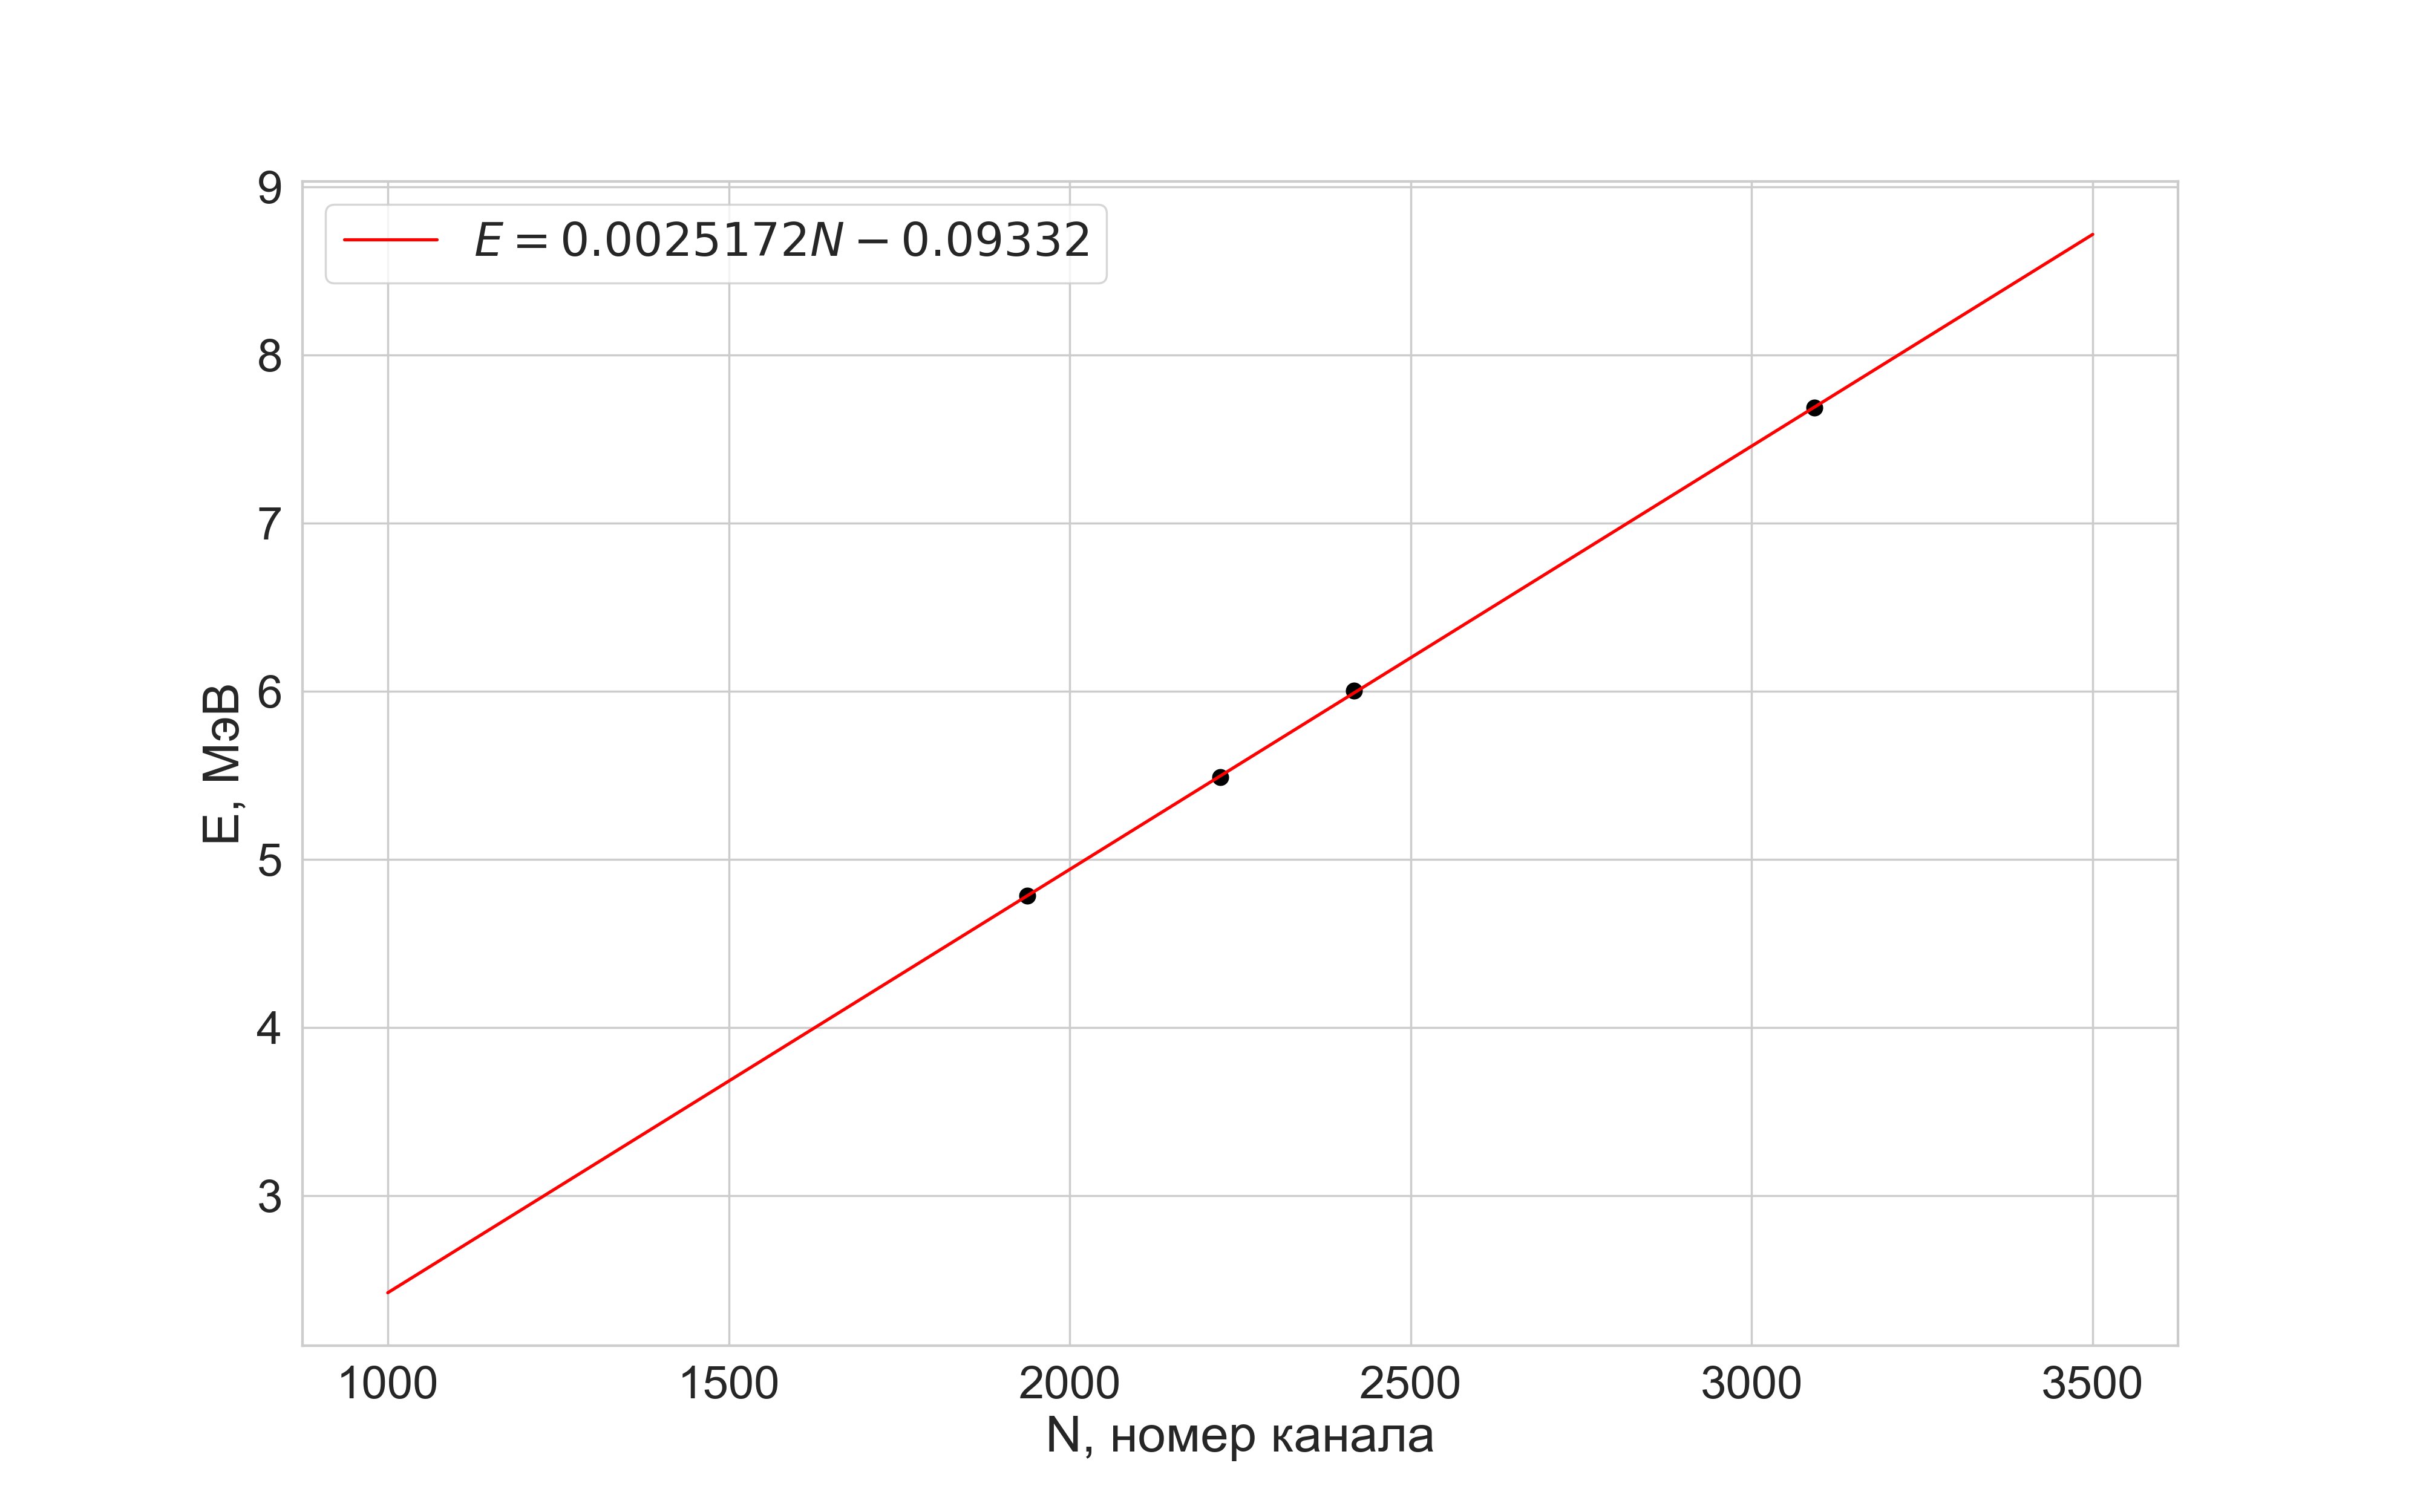
\includegraphics[width=1\textwidth]{plot_calib.png}  \caption{Калибровочный график спектрометра}
	\label{fig:calib}
\end{figure}
Результаты измерений и их обработки с учетом калибровки занесем в таблицу:

\begin{table}[H]
	\centering
	\begin{tabular}{|c|c|c|c|c|c|c|}
	\hline
			                                       & $N_i$ & $\Delta N_i$ & $E_i$, МэВ & $\Delta E_i$, МэВ & $R_i$ & $R_\text{фл}, 10^{-4}$ \\ \hline
	${ }^{238} \mathrm{U}$                         & 1672  & 67           & 4,12       & 0,17              & 0,04  & 9,35                  \\ \hline
	${ }^{238} \mathrm{U}$                         & 1925  & 51           & 4,75       & 0,13              & 0,03  & 8,70                  \\ \hline
	${ }^{241} \mathrm{Am} +   ^{230} \mathrm{Th}$ & 1909  & 47           & 4,71       & 0,12              & 0,02  & 8,74                  \\ \hline
	${ }^{241} \mathrm{Am} +   ^{230} \mathrm{Th}$ & 2241  & 31           & 5,55       & 0,08              & 0,01  & 8,06                  \\ \hline
	${ }^{239} \mathrm{Pu}$                        & 2118  & 31           & 5,24       & 0,08              & 0,01  & 8,29                  \\ \hline
	${ }^{226} \mathrm{Ra}$                        & 1938  & 37           & 4,79       & 0,09              & 0,02  & 8,67                  \\ \hline
	${ }^{226} \mathrm{Ra}$                        & 2221  & 40           & 5,50       & 0,10              & 0,02  & 8,09                  \\ \hline
	${ }^{226} \mathrm{Ra}$                        & 2417  & 44           & 5,99       & 0,11              & 0,02  & 7,75                  \\ \hline
	${ }^{226} \mathrm{Ra}$                        & 3092  & 37           & 7,69       & 0,09              & 0,01  & 6,84                  \\ \hline
	\end{tabular}
\end{table}

Для проверки закона Гейгера-Нетолла построим график $T_{1/2}(1/\sqrt{E_{\alpha}})$. Времена полураспада приведем в таблице:
\begin{table}[H]
    \centering
    \begin{tabular}{|c|c|c|c|c|} \hline
        Образец & $^{226}$Ra & $^{222}$Ra & $^{218}$Po & $^{214}$Po \\ \hline
        $T_{1/2}$ & 1620 лет & 3.82 суток & 3.11 мин & 1.63 $\cdot 10^{-4}$ с \\ \hline
    \end{tabular}
    \caption{Время полураспадов $^{226}$Ra и его дочерних ядер}
    \label{table:tab}
\end{table}

\begin{figure}[H]
	\centering
	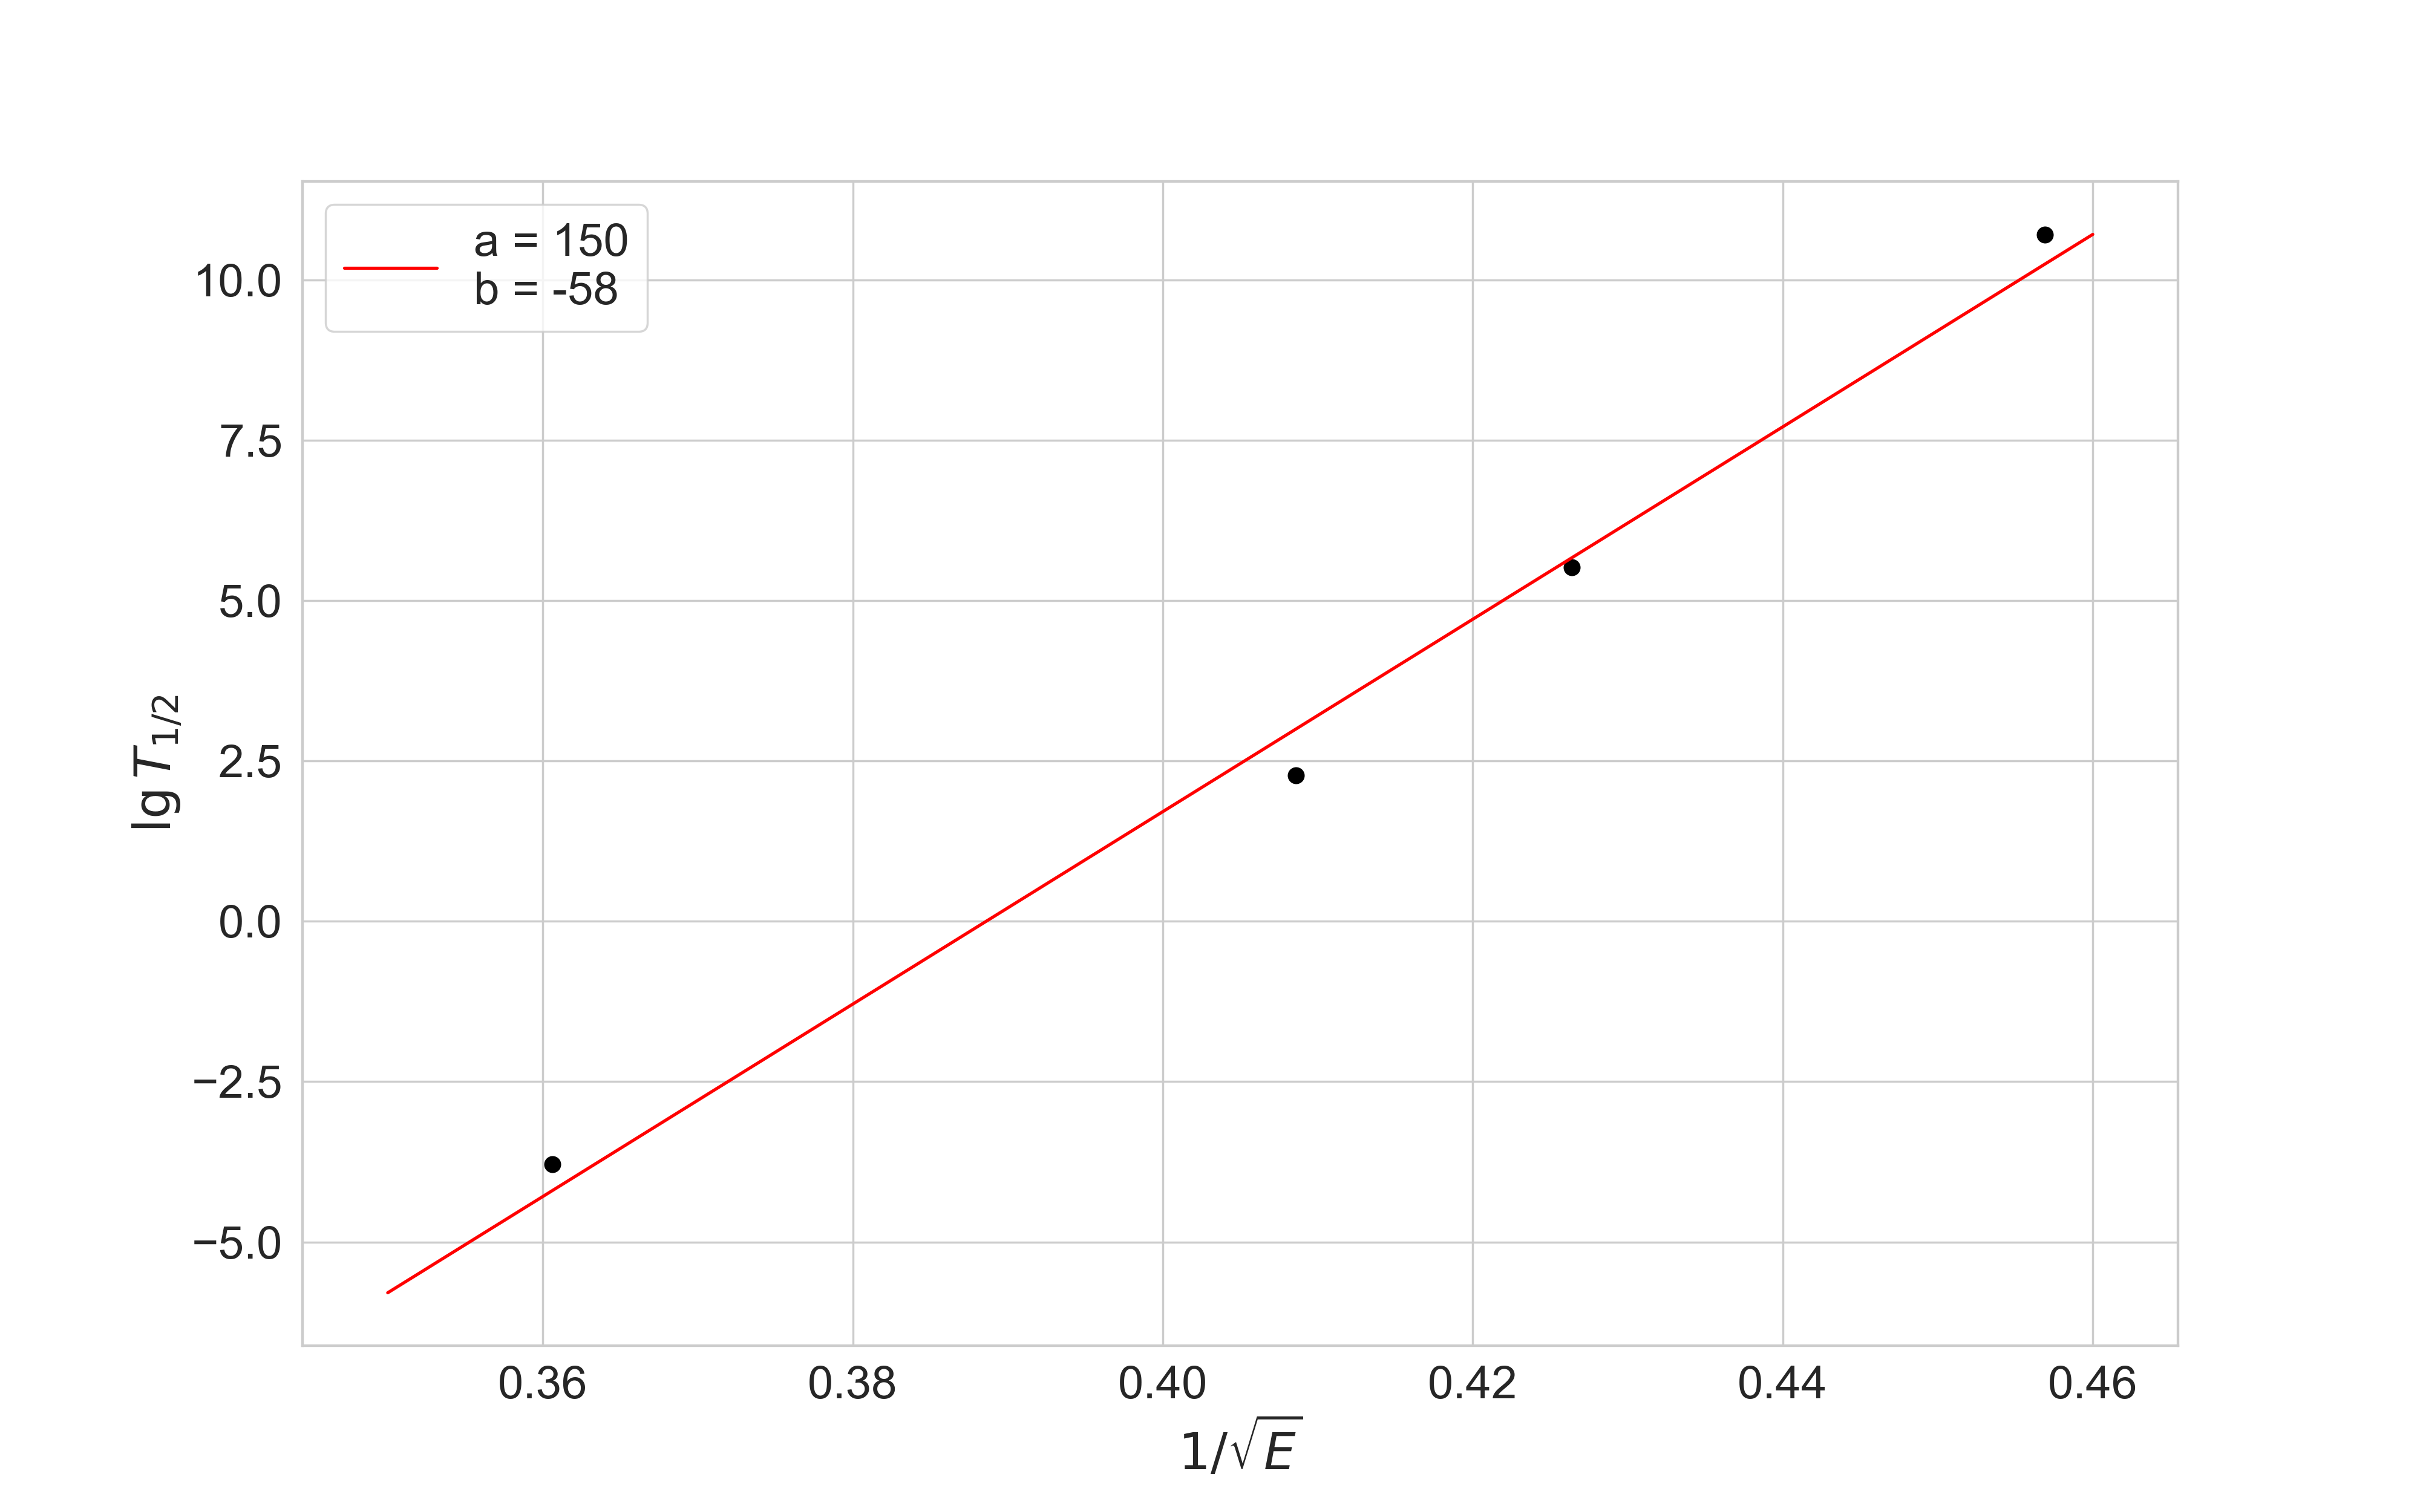
\includegraphics[width=1\textwidth]{plot_geyger.png}  \caption{График для проверки закона Гейгера - Нетолла}
	\label{fig:geyger}
\end{figure}

Отсюда коэффициенты $a$ и $b$:
\begin{align*}
    a = 150 \pm 10\\
    b = -58 \pm 5
\end{align*}

Оценка данных коэффициентов из формул:
\begin{gather*}
    a \approx 1.6Z  = 141 \\
    b \approx -1.6Z^{2/3} - 21.4 = -53
\end{gather*} 

\section{Выводы}
В ходе работы были проведены измерения спектров $\alpha$-излучения, были получены энергии $\alpha$-распадов для разных веществ. Также был проверен закон Гейгера-Нетолла связывающий период полураспада с энергией излучения. Коэффициенты совпадают с теоретическими, график действтительно имеет вид прямой.

\end{document}